\documentclass[professionalfonts]{beamer}
\usepackage{iftex,ifxetex}
\ifPDFTeX
  \usepackage[utf8]{inputenc}
  \usepackage[T1]{fontenc}
  \usepackage{lmodern}
\else
  \ifluatex
    \usepackage{unicode-math} 
    \defaultfontfeatures{Ligatures=TeX}
    % \setmathfont{Latin Modern Math}
    \setsansfont{CMU Sans Serif}
    % \setsansfont{Linux Biolinum O}
  \fi
\fi

\mode<presentation>
{
  \usetheme{Madrid}
  % or ...
  \setbeamertemplate{bibliography item}{}
  \setbeamercovered{transparent}
  % or whatever (possibly just delete it)
}

% \AtBeginSection[]{
%   \begin{frame}
%   \vfill
%   \centering
%   \begin{beamercolorbox}[sep=8pt,center,shadow=true,rounded=true]{title}

%     \usebeamerfont{title}\insertsectionhead\par%
%   \end{beamercolorbox}
%   \vfill
%   \end{frame}
% }

% \usepackage{fontspec}
\usepackage[english]{babel}
% or whatever
\usepackage{csquotes}
\usepackage[backend=biber,
        style=unified,
        maxcitenames=3,
        maxbibnames=99,
        natbib,
        url=false]{biblatex}
\addbibresource{Dissertation.bib}
% \setmainfont{Linux Libertine O}
% \setmonofont{CMU Typewriter Text}
\renewcommand{\ttdefault}{cmtt}

% \usepackage[colorlinks,allcolors={black},urlcolor={blue}]{hyperref} %allows for hyperlinks and pdf bookmarks 
\usepackage{pifont} %Maths
\usepackage{graphicx}	%Inserting graphics, pictures, images 		
\usepackage{multicol} %Multicolumn text
\usepackage{multirow} %Useful for combining cells in tablesbrew 
\usepackage{booktabs} %Enhanced tables
\usepackage{longtable}
% \usepackage{underscore} %Allows for underscores in text mode
% \usepackage[colorlinks,allcolors={black},urlcolor={blue}]{hyperref} %allows for hyperlinks and pdf bookmarks
\usepackage{url} %allows for urls
\def\UrlBreaks{\do\/\do-} %allows for urls to be broken up
% \usepackage[normalem]{ulem} %strike out text. Handy for syntax
% \usepackage{tcolorbox}
% \usepackage{datetime2}
% \usepackage{caption}
% \usepackage{subcaption}
% \usepackage{tipa} %IPA symbols
% \usepackage{tipauni}
\usepackage{langsci-gb4e} % Language Science Press' modification of gb4e
\usepackage{tikz} % Drawing Hasse diagrams
\usetikzlibrary{decorations.pathreplacing}
% \usepackage{leipzig} %	Offers support for Leipzig Glossing Rules
\usepackage{datetime2} % Date and time formatting

%%MACROS
\newcommand{\sub}[1]{\textsubscript{#1}}
\newcommand{\supr}[1]{\textsuperscript{#1}}
\providecommand{\lsptoprule}{\midrule\toprule}
\providecommand{\lspbottomrule}{\bottomrule\midrule}
\newcommand{\fittable}[1]{\resizebox{\textwidth}{!}{#1}}
\newcommand{\cmark}{\ding{51}}%


\title[Voice Quality in SLZ] % (optional, use only with long paper titles)
{Voice Quality and Laryngeal Complexity in Santiago Laxopa Zapotec}

% \subtitle{Include Only If Paper Has a Subtitle}

\author[Brinkerhoff] % (optional, use only with lots of authors)
{Mykel Loren Brinkerhoff}
% - Give the names in the same order as the appear in the paper.
% - Use the \inst{?} command only if the authors have different
%   affiliation.

\institute[UC Santa Cruz] % (optional, but mostly needed)
{University of California, Santa Cruz}
% - Use the \inst command only if there are several affiliations.
% - Keep it simple, no one is interested in your street address.

\date[2025-06-06] % (optional, should be abbreviation of conference name)
{6 June 2025}
% - Either use conference name or its abbreviation.
% - Not really informative to the audience, more for people (including
%   yourself) who are reading the slides online

% \subject{Theoretical Computer Science}
% This is only inserted into the PDF information catalog. Can be left
% out. 

% If you have a file called "university-logo-filename.xxx", where xxx
% is a graphic format that can be processed by latex or pdflatex,
% resp., then you can add a logo as follows:

\pgfdeclareimage[height=0.5cm]{university-logo}{images/UCSC_Logo_RGB.png}
\logo{\pgfuseimage{university-logo}}



% Delete this, if you do not want the table of contents to pop up at
% the beginning of each subsection:
\AtBeginSubsection[]
{
  \begin{frame}<beamer>{Outline}
    \tableofcontents[currentsection,currentsubsection]
  \end{frame}
}


% If you wish to uncover everything in a step-wise fashion, uncomment
% the following command: 

% \beamerdefaultoverlayspecification{<+->}


\begin{document}

\begin{frame}
  \titlepage
\end{frame}

\begin{frame}{Outline}
  \tableofcontents
  % You might wish to add the option [pausesections]
\end{frame}


% Structuring a talk is a difficult task and the following structure
% may not be suitable. Here are some rules that apply for this
% solution: 

% - Exactly two or three sections (other than the summary).
% - At *most* three subsections per section.
% - Talk about 30s to 2min per frame. So there should be between about
%   15 and 30 frames, all told.

% - A conference audience is likely to know very little of what you
%   are going to talk about. So *simplify*!
% - In a 20min talk, getting the main ideas across is hard
%   enough. Leave out details, even if it means being less precise than
%   you think necessary.
% - If you omit details that are vital to the proof/implementation,
%   just say so once. Everybody will be happy with that.
%-----------------------------------------------------------
\section{Introduction}
%-----------------------------------------------------------
%-----------------------------------------------------------
\subsection{Overview of my dissertation}
%-----------------------------------------------------------

\begin{frame}{Research Overview}
  \begin{block}{Overview:}
    This presentation explores what characterizes voice quality in a Santiago Laxopa Zapotec (SLZ), how is it is structured acoustically, and how this structure helps explain SLZ's laryngeal complexity.  
  \end{block}
\end{frame}

\begin{frame}{Research Overview}
  \begin{block}{Research Questions:}
    \begin{itemize}
      \item How is phonation's acoustic space structured in a single language?
      \item Which measures are important for capturing phonation contrasts?
      \item How do these measures help explain SLZ's laryngeal complexity?
    \end{itemize}
  \end{block}
\end{frame}

\begin{frame}{Research Overview}
  \begin{block}{Answers to Research Questions:}
    \begin{itemize}
      \item The acoustic space is three-dimensional and correlated with glottal-airflow (D1/D3) and nonmodal-to-modal (D2) continua.
      \item Only a handful of measures are needed for capturing contrasts.
      \item SLZ's laryngeal complexity is weakly articulated and shows phasing. 
    \end{itemize}  
  \end{block}
\end{frame}

%-----------------------------------------------------------
\subsection{What is Voice Quality?}
%-----------------------------------------------------------

\begin{frame}{What is Voice Quality?}
  \begin{itemize}
  \item Broad sense $=$ long-term characteristics of an individual's voice \citep{abercrombieElementsGeneralPhonetics1967,laverPhoneticDescriptionVoice1980}.
  \item Narrow sense $=$ how larynx affects phonetic characteristics of speech sounds \citep[e.g.,][]{eslingVoiceQualityLaryngeal2019}.
  \item Sometimes used interchangeably with phonation
    \begin{itemize}
      \item \cite{barzilaiContextdependentPhoneticEnhancement2021} use \textit{voice quality} for phonetic description and \textit{phonation} for phonological contrasts.
    \end{itemize}
  \end{itemize}
\end{frame}

\begin{frame}{How is voice quality used?}
  \begin{itemize}
    \item Paralinguistic information by ``indexing the biological, psychological, and social characteristics of the speaker'' \citep[e.g.,][]{laverVoiceQualityIndexical1968,podesvaStanceWindowLanguageRace2016}
    \item Phonological contrasts \citep[e.g.,][]{espositoCrosslinguisticPatternsPhonation2020}.
    \begin{itemize}
      \item Gujarati's breathy and modal vowels \citep{fischer-jorgensenPhoneticAnalysisBreathy1968}.
      \item Mazatec's breathy, creaky, and modal vowels \citep{silvermanLaryngealComplexityOtomanguean1997}.
    \end{itemize}
  \end{itemize}
\end{frame}

% \begin{frame}{Why study voice quality?}
%   \begin{itemize}
%     \item Voice quality plays a crucial role in speech communication.
%     \item It is used in many languages to create phonological contrasts.
%     \item It is a rich area of research that can help us understand speech production and perception.
%   \end{itemize}
% \end{frame}

%-----------------------------------------------------------
\subsection{Santiago Laxopa Zapotec}
%-----------------------------------------------------------

\begin{frame}{What is Santiago Laxopa Zapotec}
  \begin{columns}
    \begin{column}{0.33\textwidth}
      \begin{itemize}
        \item Santiago Laxopa Zapotec (SLZ; \textit{Dille'xhunh Laxup}) is a Sierra Norte variety of Zapotec (Oto-Manguean).
        \item Spoken by c. 1,000 speakers in Santiago Laxopa and in diaspora.
      \end{itemize}
    \end{column}
    \begin{column}{0.67\textwidth}
      \begin{figure}
        \centering
        \includegraphics[width=0.95\linewidth]{images/Oaxaca_Santiago_Laxopa_Map.eps}
      \end{figure}
    \end{column}
  \end{columns}
\end{frame}

\begin{frame}{Why study SLZ?}
  \begin{itemize}
        \item SLZ is a relatively understudied language
        \begin{itemize}
          \item Contributes to our understanding of language diversity.
          \item Test claims about language.
        \end{itemize}
    \item SLZ has a complex laryngeal system that has not been fully documented.
    \begin{itemize}
      \item SLZ has a four-way phonation contrast.
      \item SLZ has a five-way tonal contrast.
      \item These contrasts are orthogonal, meaning that they can occur independently of each other.
    \end{itemize} 
  \end{itemize}
\end{frame}

\begin{frame}{Phonation in SLZ}
  \begin{itemize}
    \item SLZ has a four-way phonation contrast:
    \begin{itemize}
      \item Modal ( [ a ] )
      \item Breathy ( [ a̤ ] )
      \item Checked ( [aʔ] or [ aa̰ ] )
      \item Rearticulated ([ aʔa ], [ aa̰a ], or [ a̰ ] )
    \end{itemize}
  \end{itemize}
\end{frame}

\begin{frame}{Breathy Phonation in SLZ}
  \begin{columns}
    \begin{column}{0.33\linewidth}
      \begin{itemize}
        \item Characterized by aperiodicity and noise in the harmonic structure.
        \item Longer duration than modal voice
        \item Lower fundamental frequency (\textit{f}0)
      \end{itemize}  
    \end{column}
    \begin{column}{0.67\linewidth}
      \begin{figure}
        \centering
        \includegraphics[width=\textwidth]{images/Spectrograms/yah.png}
      \end{figure}
    \end{column}
  \end{columns}
\end{frame}

\begin{frame}{Checked Phonation in SLZ}
  \begin{columns}
    \begin{column}{0.33\linewidth}
      \begin{itemize}
        \item Glottal occlusion at the end of vowel or creaky voice in second half vowel.
        \item Decrease in voicing amplitude during second half.
      \end{itemize}  
    \end{column}

    \begin{column}{0.67\linewidth}
      \begin{figure}
        \centering
        \includegraphics[width=\textwidth]{images/Spectrograms/RD_yu'.png}
      \end{figure}
    \end{column}
  \end{columns}
\end{frame}

\begin{frame}{Rearticulated Phonation in SLZ}
  \begin{columns}
    \begin{column}{0.33\linewidth}
      \begin{itemize}
        \item Glottal occlusion or creaky voice in the middle of the vowel.
        \item Longer duration than modal voice
        \item Decrease in voicing amplitude during first half.
      \end{itemize}  
    \end{column}

    \begin{column}{0.67\linewidth}
      \begin{figure}
        \centering
        \includegraphics[width=\textwidth]{images/Spectrograms/xa'ag.png}
      \end{figure}
    \end{column}
  \end{columns}
\end{frame}

\begin{frame}{Tone in SLZ}
  \begin{itemize}
    \item SLZ shows a five-way tonal contrast on monosyllabic nouns \citep{brinkerhoffTonalPatternsTheir2022}.
  \end{itemize}
  \begin{center}
    \begin{tabular}{llll}
      \lsptoprule
      \textbf{Tone} & \textbf{Example} & \textbf{Transcription} & \textbf{Gloss} \\
      \midrule
      High    &  \textit{xha}   &  [ ʐa˦ ] & `clothing.poss'\\
      Mid     &  \textit{lhill} & [ ɾiʒ˧ ] & `house.poss' \\
      Low     &  \textit{yu'}   & [ çuˀ˨ ] & `earth'\\
      Rising  &  \textit{yu'u}  & [ çuˀu˧˦ ] & `lime (Sp. \textit{cal})' \\
      Falling &  \textit{yu'u}  & [ çuˀu˦˨ ] & `house' \\
      \lspbottomrule
    \end{tabular}
  \end{center}
\end{frame}

\begin{frame}{Interaction of Tone and Phonation in SLZ}
  \begin{itemize}
    \item Tone and phonation are orthogonal.
  \end{itemize}
  \begin{center}
    \begin{tabular}{lcccc}
      \lsptoprule
      & \textbf{Modal} & \textbf{Breathy} & \textbf{Checked} & \textbf{Rearticulated} \\
      \midrule
      High    & \cmark & -- & \cmark & \cmark \\
      Mid     & \cmark & \cmark & \cmark & \cmark \\
      Low     & \cmark & \cmark & \cmark & \cmark \\
      Rising  & \cmark & \cmark & -- & \cmark \\
      Falling & \cmark & \cmark & \cmark & \cmark \\
      \lspbottomrule
    \end{tabular}
  \end{center}
\end{frame}

%-----------------------------------------------------------
\section{Previous research}
%-----------------------------------------------------------
% \frame{\sectionpage}
%-----------------------------------------------------------
\subsection{Measuring Voice Quality}
%-----------------------------------------------------------

\begin{frame}{Measuring voice quality}
  \begin{itemize}
    \item Long been established that phonation has correlates in the acoustic signal (e.g., \cite{fischer-jorgensenPhoneticAnalysisBreathy1968,klattAnalysisSynthesisPerception1990}).
    \item \citet{fischer-jorgensenPhoneticAnalysisBreathy1968} found that a strengthened fundamental (i.e., H1) correlated with breathy vowels in Gujarati.
    \begin{itemize}
      \item Proposed H1$-$H2 amplitude as a measure to normalize for overall intensity differences
    \end{itemize}
    \item Subsequent research shows H1$-$H2 is useful for classifying voice quality contrasts.  
    \item However, it is not without its problems (see \cite{chaiH1H2AcousticMeasure2022} for an overview).
  \end{itemize}
\end{frame}

\begin{frame}{Measuring voice quality}
  \begin{itemize}
    \item H2 and other normalizations (A1, A3) are really attempts to understand the relative strength of the fundamental (H1) to higher harmonic energy
    \item H1 and H2 are affected by subglottal pressure differently \citep{sundbergObjectiveCharacterizationPhonation2022}
    \begin{itemize}
      \item This undermines the original reasoning behind H1$-$H2
    \end{itemize} 
    \item Researchers sometimes find that H1$-$H2 does not distinguish phonation types \citep[e.g.,][]{espositoVariationContrastivePhonation2010,espositoAcousticElectroglottographicStudy2012,garellekPhoneticsWhiteHmong2023}.
    \item Error in measuring H1$-$H2 is uncomfortably high \citep[e.g.,][]{chaiH1H2AcousticMeasure2022}.
  \end{itemize}
\end{frame}

\begin{frame}{Measuring voice quality}
  \begin{itemize}
    \item Many measures have been proposed to capture voice quality.
    \item Measures can be broadly categorized into several categories \citep{gordonPhonationTypesCrosslinguistic2001}:
    \begin{itemize}
      \item Periodicity (e.g., HNR or CPP)
      \item Energy 
      \item Spectral tilt (e.g., H1*$-$H2*, residual H1*)
      \item Pitch (e.g., \textit{f}0)
      \item Duration 
    \end{itemize}
  \item Linguists have used combinations of these measures to model phonation (e.g., \cite{blankenshipTimingNonmodalPhonation2002,brunelleTonePhonationSoutheast2016,espositoAcousticElectroglottographicStudy2012}).
  \end{itemize}
\end{frame}

\begin{frame}{New measures of voice quality}
  \begin{itemize}
    \item New measures are being developed all the time.
    \item \posscitet{chaiH1H2AcousticMeasure2022} residual H1* is a new measure of spectral tilt that is more robust than traditional spectral tilt measures.
    \begin{itemize}
      \item Does this by removing the the effects of Energy from the H1* measure.
      \item This was the original goal of \citet{fischer-jorgensenPhoneticAnalysisBreathy1968}
    \end{itemize}
    \item \citet{brinkerhoffUsingResidualH12025} found that residual H1* is a better measure of spectral tilt than H1*$-$H2* for SLZ.
  \end{itemize}
\end{frame}

\begin{frame}{Too many measures}
  \begin{itemize}
    \item There are many measures of voice quality, but it is not clear which ones are the most useful.
    \item It also makes it difficult to compare results across studies.
    \item VoiceSauce makes this a common issue \citep{shueVoiceSauceProgramVoice2011}.
    \begin{itemize}
      \item Computes almost every acoustic measure related to voice quality.
      \item Many of these measures are potentially redundant (e.g., three different algorithms for calculating $f0$, formants, and bandwidths). 
      \item Hard to know which measures to focus on.
    \end{itemize}
  \end{itemize}
\end{frame}

\begin{frame}{Too many measures}
  \begin{itemize}
    \item \citet{kreimanUnifiedTheoryVoice2014,kreimanValidatingPsychoacousticModel2021} tackle this by proposing a psychoacoustic model of voice quality.
    \item Found certain measures are perceptually more important than others.
  \end{itemize}
  \begin{center}
    \fittable{
    \begin{tabular}{ll}
      \lspbottomrule
      \textbf{Model Component} & \textbf{Parameters} \\
      \midrule
      \multirow{4}{*}{Harmonic source spectral shape} 
        & H1--H2 \\
        & H2--H4 \\
        & H4--2~kHz \\
        & 2~kHz--5~kHz \\
      \midrule
      Inharmonic source excitation 
        & Spectrally-shaped noise-to-harmonics ratio \\
      \midrule
      \multirow{2}{*}{Time-varying source characteristics} 
        & $f0$ mean and standard deviation (or $f0$ track) \\
        & Amplitude mean and standard deviation (or amplitude track) \\
      \midrule
      \multirow{2}{*}{Vocal tract transfer function} 
        & Formant frequencies/bandwidths \\
        & Spectral zeroes/bandwidths \\
      \lspbottomrule
    \end{tabular}}
  \end{center}
\end{frame}

%-----------------------------------------------------------
\subsection{Modeling Voice Quality}
%-----------------------------------------------------------


\begin{frame}{Modeling voice quality}
  \begin{itemize}
    \item Early models proposed that voice quality is one dimensional and represents glottal airflow \citep{ladefogedPreliminariesLinguisticPhonetics1971,ladefogedSoundsWorldsLanguages1996}.
  \end{itemize}
  \begin{figure}[h]
    % \centering
    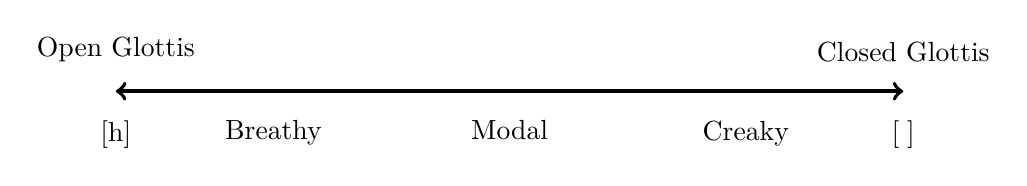
\begin{tikzpicture}
        % Draw the line with arrows at both ends
        \draw[<->, line width=0.5mm] (0,0) -- (10,0);
        
        % Labels underneath the line
        \node[below, yshift=-0.25cm] at (0,0) {[h]};
        \node[below, yshift=-0.25cm] at (2,0) {Breathy};
        \node[below, yshift=-0.25cm] at (5,0) {Modal};
        \node[below, yshift=-0.25cm] at (8,0) {Creaky};
        \node[below, yshift=-0.25cm] at (10,0) {[ʔ]};
        
        % Labels above the line
        \node[above, yshift=0.25cm] at (0,0) {Open Glottis};
        \node[above, yshift=0.25cm] at (10,0) {Closed Glottis};
    \end{tikzpicture}
  \end{figure}
\end{frame}

\begin{frame}{Voice quality's multidimensionality}
  \begin{itemize}
    \item More recent work has shown that voice quality is not one-dimensional, but minimally five-dimensional \citep[e.g.,][]{garellekModelingVoiceSource2016,kreimanValidatingPsychoacousticModel2021}.
    \begin{itemize}
      \item Especially in the case of individual speaker differences.
    \end{itemize}
    \item \citet{garellekVoiceQualityTone2013} has argued that dimensionality might not be as complex for capturing phonation contrasts.
  \end{itemize}
\end{frame}

\begin{frame}{\citet{keatingCrosslanguageAcousticSpace2023}}
  \begin{itemize}
    \item Explored phonation's cross-linguistic acoustic space.
    \item Found a two-dimensional space for phonation across 11 languages.
    \begin{enumerate}
      \item First dimension $=$ nonmodal-to-modal continuum.
      \item Second dimension $=$ glottal-airflow continuum.
    \end{enumerate}
    \item Found languages with more contrasts used more of the acoustic space than languages with fewer contrasts.
    \item Found correlations between dimensions and acoustic measures.
    \begin{enumerate}
      \item First dimension $=$ periodicity and energy measures.
      \item Second dimension $=$ spectral tilt and periodicity measures.
    \end{enumerate}
  \end{itemize}
\end{frame}

\begin{frame}{\citet{keatingCrosslanguageAcousticSpace2023}}
  \begin{columns}
    \begin{column}{0.3\linewidth}
      \begin{itemize}
        \item Colors $=$ phonation.
        \item Labels $=$ language and phonation.
      \end{itemize}
    \end{column}
    \begin{column}{0.7\linewidth}
      \begin{figure}
        \includegraphics[width=.8\linewidth]{images/Keating_dimension.png}
        \caption{Figure 4 from \citet{keatingCrosslanguageAcousticSpace2023}.}
      \end{figure}
    \end{column}
  \end{columns}
\end{frame}

%-----------------------------------------------------------
\section{My Analyses}
%-----------------------------------------------------------
%-----------------------------------------------------------
\subsection{Data and Methods}
%-----------------------------------------------------------
\begin{frame}{Data}
  \begin{itemize}
    \item Data comes from SLZ fieldwork from Summer 2022.
    \item Production data was collected from 10 speakers (5 male/5 female).
    \item Recordings were made in a quiet room using a Zoom H4n Pro handheld recorder (16-bit, 44.1 kHz).
  \end{itemize}
\end{frame}
\begin{frame}{Methods}
  \begin{itemize}
    \item Participants produced 72 words in a carrier phrase 3 times each.
    \begin{itemize}
      \item \textit{Shnia' X chonhe lhas} [ʃnːiaˀ X tʃone ɾas] ``I say X three times.''
    \end{itemize}
    \item Words covered the four-way phonation contrast.
    \item Tone was not balanced due to frequency constraints. 
  \end{itemize}
  \begin{center}
  \begin{tabular}{llllll}
    \lsptoprule
    & High & Mid & Low & Rising & Falling\\
    \midrule
    Modal & 14 & 9 & 15 & 2 & 10 \\
    Breathy & $-$ & $-$ & 11 & $-$ & 2 \\
    Checked & 1 & $-$ & 9 & $-$ & \\
    Rearticulated & 1 & $-$ & 4 & $-$ & 4 \\
    \lspbottomrule
  \end{tabular}
  \end{center}
\end{frame}

\begin{frame}{Methods}
  \begin{itemize}
    \item Vowels were segmented in Praat from the second glottal pulse to the last glottal pulse before the drop in amplitude \citep{garellekAcousticDiscriminabilityComplex2020}
    \item Acoustic measures were extracted using VoiceSauce \citep{shueVoiceSauceProgramVoice2011}.
  \end{itemize}
\end{frame}

\begin{frame}{Data cleaning}
  \begin{itemize}
    \item All acoustic measures were normalized by speaker.
    \item Outliers were removed using the following criteria:
    \begin{itemize}
      \item If the z-scored $f0$ was greater than 3 or less than -3.
      \item If Energy was equal to 0.
      \item If the Mahalanobis distance was greater than 6 in the F1-F2 panel for each vowel category.
    \end{itemize}
    \item Calculated residual H1* \citep{chaiH1H2AcousticMeasure2022}.
  \end{itemize}
\end{frame}

%-----------------------------------------------------------
\subsection{Acoustic Landscape Analysis}
%-----------------------------------------------------------

\begin{frame}{MDS analysis}
  \begin{itemize}
    \item Multidimensional scaling (MDS; \cite{kruskalMultidimensionalScaling1978}) is a dimensionality reduction technique.
    \item Used to visualize the structure of a high-dimensional space in a lower-dimensional space.
    \item Especially effective when many variables contribute to the structure of the space.
    \item More robust than principal component analysis (PCA) or linear discriminant analysis (LDA) because it does not assume linearity or normality of the data.
  \end{itemize}
\end{frame}

\begin{frame}{Predictions for the MDS analysis}
  \begin{itemize}
    \item Small number of dimensions needed to capture the structure of the space.
    \item Phonation types will occupy distinct regions of the space.
    \item Dimensions should be comparable to those found in \citet{keatingCrosslanguageAcousticSpace2023}.
    \item Dimensions should show correlations with acoustic measures.
  \end{itemize}
\end{frame}

\begin{frame}{Number of Dimensions needed}
  \begin{figure}
    \centering
    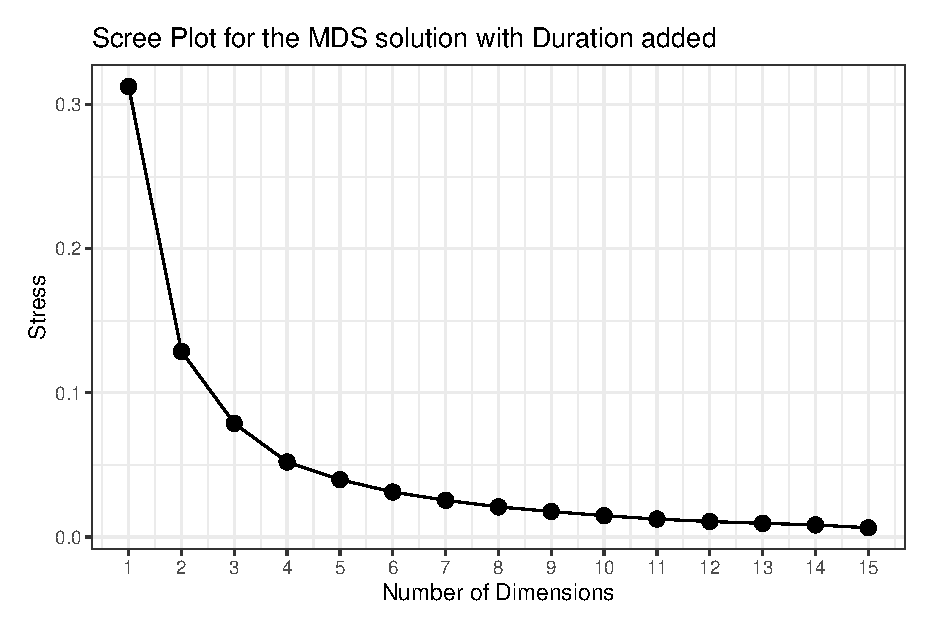
\includegraphics[width = 0.8\linewidth]{images/MDS/stress_plot_dur.eps}
\end{figure}
\end{frame}

\begin{frame}{Explanation of the plots}
  \begin{itemize}
    \item Each point $=$ unique speaker x phonation combination.
    \item Colors $=$ phonation type.
    \begin{itemize}
      \item Modal $=$ black
      \item Breathy $=$ orange
      \item Checked $=$ blue
      \item Rearticulated $=$ green
    \end{itemize}
    \item Axes $=$ dimensions of the acoustic space.
  \end{itemize}
\end{frame}

\begin{frame}{Dimensionality in SLZ}
  \begin{itemize}
    \item Scan the QR code to see the three-dimensional space.
    \item Or use the link: \href{https://bit.ly/3St9S6g}{https://bit.ly/3St9S6g}
  \end{itemize}
  \begin{figure}
    \centering
    \includegraphics[width=5cm, scale=0.5]{qrcode_3d_plot.eps}
  \end{figure}
\end{frame}

\begin{frame}{Takeaways from 3D plot}
  \begin{itemize}
    \item Occupies a three-dimensional space.
    \item Clear groupings of phonation types.
    \item Very little overlap between phonation types.
  \end{itemize}
\end{frame}

\begin{frame}{Dimensionality in SLZ}
  \begin{figure}
    \centering
    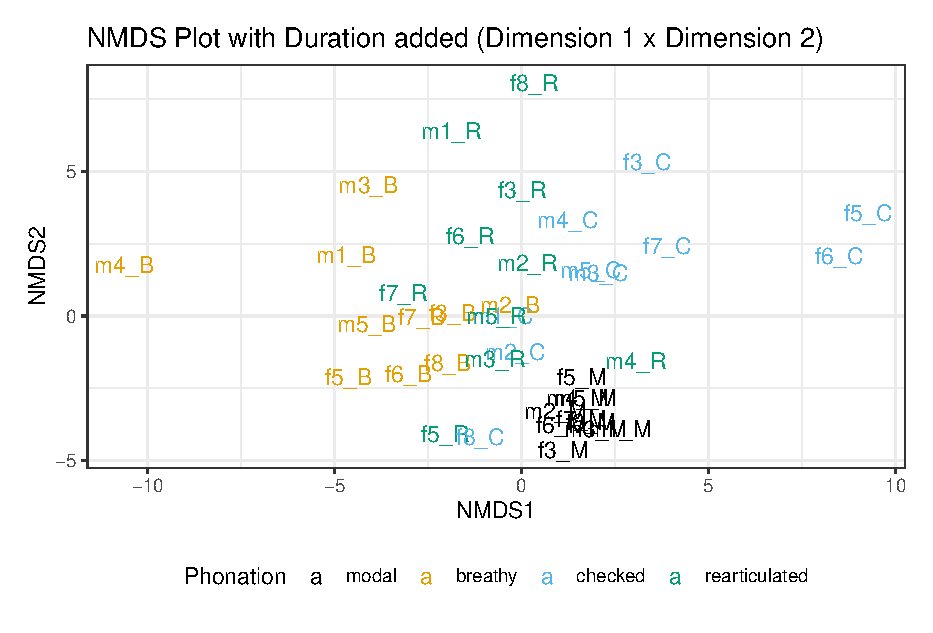
\includegraphics[width = 0.8\linewidth]{images/MDS/nmds12_dur.eps}
  \end{figure}
\end{frame}

\begin{frame}{Dimensionality in SLZ}
  \begin{figure}
    \centering
    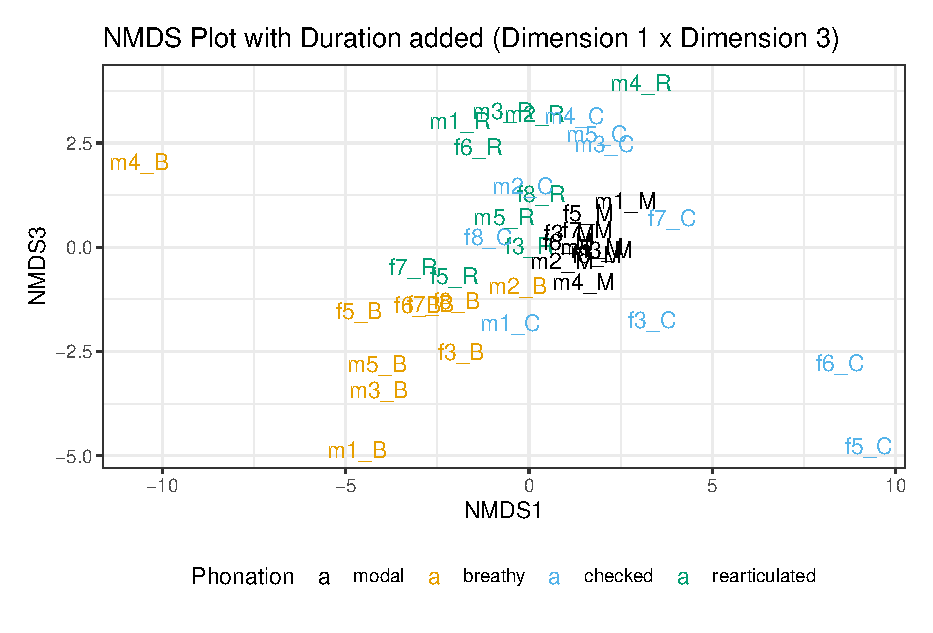
\includegraphics[width = 0.8\linewidth]{images/MDS/nmds13_dur.eps}
  \end{figure}
\end{frame}

\begin{frame}{Dimensionality in SLZ}
  \begin{figure}
    \centering
    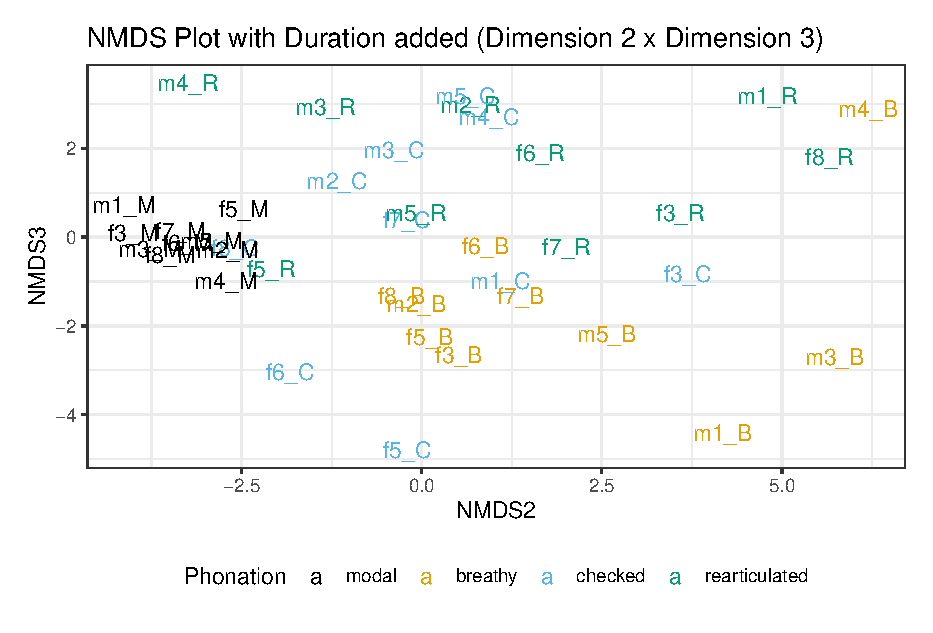
\includegraphics[width = 0.8\linewidth]{images/MDS/nmds23_dur.eps}
  \end{figure}
\end{frame}

\begin{frame}{Summary of Dimensions}
  \begin{itemize}
    \item Dimension 1 (D1) gives a rough continuum from breathy to creaky.
    \item Dimension 2 (D2) gives a rough continuum from modal to nonmodal.
    \item Dimension 3 (D3) gives a rough continuum from breathy to creaky.
  \end{itemize}
\end{frame}

\begin{frame}{Correlation to Acoustic Measures}
  \begin{itemize}
    \item D1 correlated with spectral tilt measures: 
    \begin{itemize}
      \item H1*$-$A1* ($r^2 = -0.83$) 
      \item H1*$-$A2* ($r^2 = -0.86$)
      \item H1*$-$A3* ($r^2 = -0.81$)
    \end{itemize}
    \item D2 correlated with periodicity and energy: 
    \begin{itemize}
      \item HNR\textless 500 Hz ($r^2 = -0.79$)
      \item HNR\textless 1500 Hz ($r^2 = -0.80$)
      \item Energy ($r^2 = -0.79$)
    \end{itemize}
    \item D3 correlated with different spectral tilts:
    \begin{itemize}
      \item residual H1* ($r^2 = -0.72$)
      \item H2*$-$H4* ($r^2 = -0.69$)
      \item H2* ($r^2 = -0.68$)
    \end{itemize}
  \end{itemize}
\end{frame}

\begin{frame}{Summary of Acoustic Landscape}
  \begin{itemize}
    \item SLZ's phonation occupies a three-dimensional space.
    \item Dimensions are correlated with glottal-airflow continuum (D1/D3) and nonmodal-to-modal continuum (D2).
    \item Dimensions are similar to those found in \citet{keatingCrosslanguageAcousticSpace2023}.
  \end{itemize}
\end{frame}

\begin{frame}{Summary of Acoustic Landscape}
  \begin{itemize}
    \item Acoustic space can be reduced to two dimensions.
    \item More dimensions add information about these two dimensions.
  \end{itemize}
  \begin{figure}
    \centering
    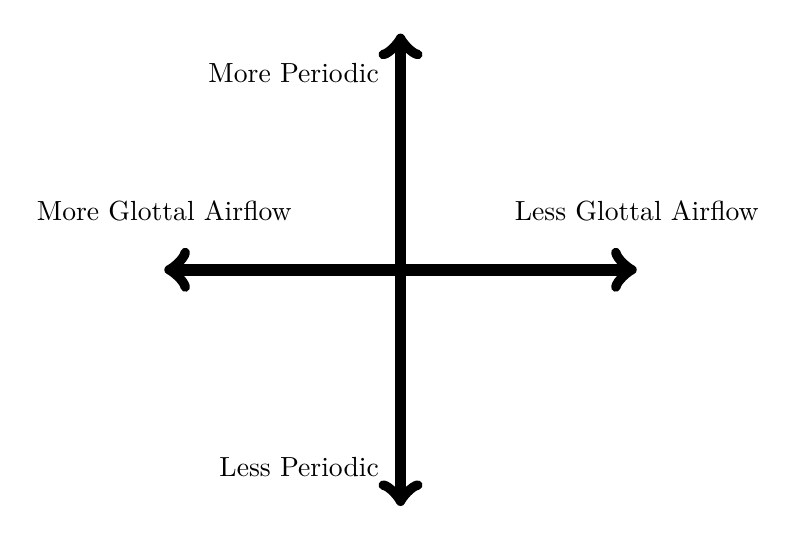
\begin{tikzpicture}
        % Draw the horizontal line with arrows
        \draw[<->, line width=1.5mm] (-3,0) -- (3,0);
        % Draw the vertical line with arrows
        \draw[<->, line width=1.5mm] (0,-3) -- (0,3);
        
        % Labels for the horizontal line
        \node[below,yshift=1cm] at (-3,0) {More Glottal Airflow};
        \node[below,yshift=1cm] at (3,0) {Less Glottal Airflow};
        
        % Labels for the vertical line
        \node[left, xshift = -1.5mm] at (0,-2.5) {Less Periodic};
        \node[left, xshift = -1.5mm] at (0,2.5) {More Periodic};
    \end{tikzpicture}
  \end{figure}
\end{frame}

%-----------------------------------------------------------
\subsection{Random Forest Analysis}
%-----------------------------------------------------------

\begin{frame}{What are decision trees?}
  \begin{columns}
    \begin{column}{0.40\linewidth}
      \begin{itemize}
        \item Decision trees are a type of statistical modeling \citep{breimanClassificationRegressionTrees1986}.
        \item Used for classification and regression tasks.
        \item Splits the data into subsets based on variable values.
        \item Splits and rules are graphically represented as a tree structure.
      \end{itemize}
    \end{column}
    \begin{column}{0.60\linewidth}
      \begin{figure}
        \centering
        \includegraphics[width=0.8\textwidth]{images/decisiontreespace.png}
        \caption{Figure 8.2 from \citet{jamesIntroductionStatisticalLearning2021}}
        % \caption[short]{title}
      \end{figure}
    \end{column}
  \end{columns}
\end{frame}

\begin{frame}{What are decision trees?}
  \begin{columns}
    \begin{column}{0.40\linewidth}
      \begin{itemize}
        \item Splits and their rules are graphically represented as a tree structure.
      \end{itemize}
    \end{column}
    \begin{column}{0.60\linewidth}
      \begin{figure}
        \centering
        \includegraphics[width=0.7\textwidth]{images/tree.png}
        \caption{Figure 8.1 from \citet{jamesIntroductionStatisticalLearning2021}}
      \end{figure}
    \end{column}
  \end{columns}
\end{frame}

\begin{frame}
  \frametitle{Use in linguistics}
  \begin{columns}
    \begin{column}{0.40\linewidth}
      \begin{itemize}
        \item Decision trees are not commonly used in linguistics.
        \item Used by \citet{tagliamonteModelsForestsTrees2012} for sociolinguistic variation.
        \item Used by \citet{keatingCrosslanguageAcousticSpace2023} to analyze phonation contrasts. 
        \item One issue with decision trees is \textit{high variance}.
      \end{itemize}
    \end{column}
    \begin{column}{0.67\linewidth}
      \begin{figure}
        \centering
        \includegraphics[width=.8\linewidth]{images/keating_tree.pdf}
        \caption{Figure 8 from \citet{keatingCrosslanguageAcousticSpace2023}.}
      \end{figure}
    \end{column}
  \end{columns}  
\end{frame}

\begin{frame}
  \frametitle{What are Random Forests?}
  \begin{itemize}
    \item Random forests are an extension of decision trees \citep{breimanRandomForests2001}.   
    \item Instead a single decision tree, multiple decision trees (i.e., a forest) are created.
    \item Trees trained on a random subset of the data and a random subset of the parameters.
    \item The final prediction is made by averaging the predictions of all trees.
    \item This reduces overfitting and improves accuracy.
  \end{itemize}
\end{frame}

\begin{frame}
  \frametitle{Tuning Random Forests}
  \begin{itemize}
    \item Requires tuning to find the best parameters \citep[e.g.,][]{boehmkeHandsOnMachineLearning2019}.
    \item Two important parameters need to be tuned:
    \begin{itemize}
      \item How many trees to create in the forest.
      \item How many variables to consider when splitting the data.
    \end{itemize}
  \end{itemize}
\end{frame}

\begin{frame}
  \frametitle{Tuning Random Forests}
  \begin{itemize}
    \item Tune with hyperparameter grid search \citep{boehmkeHandsOnMachineLearning2019}.
    \item Number of trees is sequence of trees up to 2000.
    \item Number of variables (i.e., $mtry$) $=$ 5\%, 15\%, 25\%, 40\%, 100\%, of the total number of variables ($p$).
    \begin{itemize}
      \item Also include $mtry = \sqrt{p}$ (default for classification tasks) and $mtry = \frac{p}{3}$ (for regression tasks) as options.
    \end{itemize}
  \end{itemize}
\end{frame}

\begin{frame}{Parameters for SLZ Analysis}
  \begin{columns}
    \begin{column}{0.2\linewidth}
      \begin{itemize}
        \item $mtry = 5$
        \item 300 trees.
      \end{itemize}
    \end{column}
    \begin{column}{0.80\linewidth}
      \begin{figure}
        \centering
        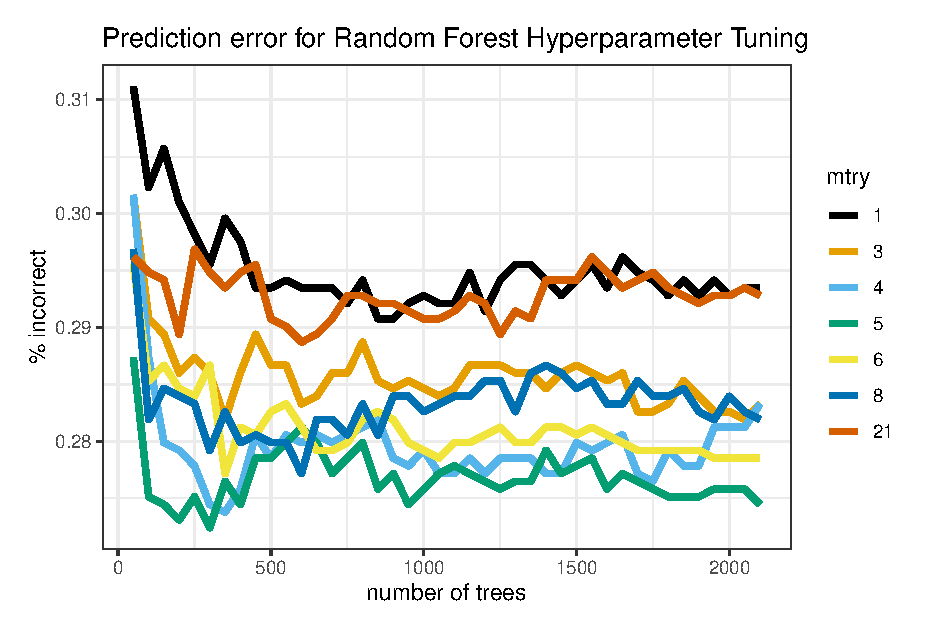
\includegraphics[width=\textwidth]{images/RandomForest/tree_num_dur.eps}
      \end{figure}
    \end{column}  
  \end{columns}
\end{frame}

\begin{frame}
  \frametitle{Interpreting Random Forests}
  \begin{itemize}
    \item Improvement in accuracy comes at the cost of interpretability.
    \item No single tree can be interpreted, but the forest as a whole.
    \item Variable importance can be calculated to determine which variables are most important for the model.
    \item Two common methods for calculating variable importance:
    \begin{itemize}
      \item How much they reduce impurity at the splits.
      \item How much the model's accuracy decreases when a variable is permuted.
    \end{itemize}
  \end{itemize}
\end{frame}

\begin{frame}
  \frametitle{Predictions for Random Forests}
  \begin{itemize}
    \item Certain measures expected to be more important than others.
    \item Should be similar to the measures found in the MDS analysis.
    \begin{itemize}
      \item Spectral tilt measures (e.g., H1*$-$A1*, residual H1*).
      \item Periodicity measures (e.g., HNR, CPP).
      \item Energy measures (e.g., Energy, SoE).
    \end{itemize}
  \end{itemize}
\end{frame}

\begin{frame}
  \frametitle{Variable Importance in SLZ}
  \begin{figure}
    \centering
    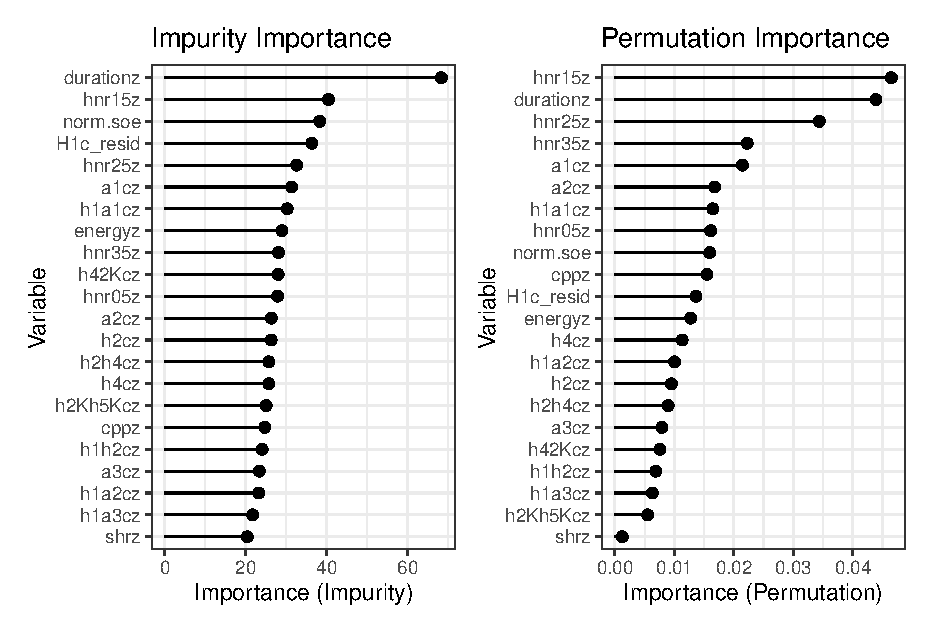
\includegraphics[width = 0.8\linewidth]{images/RandomForest/rf_dur_plots.eps}
  \end{figure}
\end{frame}

\begin{frame}{Variable Importance}
  \begin{itemize}
    \item Variable importance shows that only a handful of measures are important for capturing phonation contrasts.
    \begin{enumerate}
      \item Duration
      \item A1*
		  \item H1*$-$A1*
      \item Residual H1*
		  \item HNR < 1500 Hz
		  \item Strength of Excitation (SoE)
    \end{enumerate} 
  \end{itemize}
\end{frame}

\begin{frame}{Summary of Random Forest Results}
  \begin{itemize}
    \item Only a handful of measures are important for capturing phonation contrasts.
    \item Duration, A1*, H1*$-$A1*, residual H1*, HNR < 1500 Hz, and SoE are the most important measures.
    \item Overlap between MDS' correlated measures and the important measures from the Random Forests.
    \item Provides us with a subset of measures to use for quantifying laryngeal complexity.
    \begin{itemize}
      \item Strength of Excitation (SoE)
      \item HNR < 1500 Hz
    \end{itemize}
  \end{itemize}
\end{frame}

%-----------------------------------------------------------
\section{Laryngeal Complexity in SLZ}
%-----------------------------------------------------------

%-----------------------------------------------------------
\subsection{What is Laryngeal Complexity}
%-----------------------------------------------------------

\begin{frame}{What is Laryngeal Complexity}
  \begin{itemize}
    \item \textit{Laryngeal complexity} describes languages that use both contrastive tone and phonation \citep{silvermanLaryngealComplexityOtomanguean1997,silvermanPhasingRecoverability1997}.
    \item Very common in the Oto-Manguean language family, but is also found in other languages.
  \end{itemize}
\end{frame}

\begin{frame}{Phonation's phasing}
  \begin{itemize}
    \item One of the key features of laryngeal complexity is \textit{phasing}.
    \item To maximize production and perception constraints, tone and phonation are not produced simultaneously, but rather in sequence.
    \item This produces a complex segment that has a modal portion for tone and a nonmodal portion for phonation.
    \item There are three types of phasing:
    \begin{itemize}
      \item \textit{Prevocalic} phasing $=$ phonation is produced before modal portion.
      \item \textit{Postvocalic} phasing $=$ phonation is produced after modal portion.
      \item \textit{Interrupted} phasing $=$ phonation is produced in the middle of the modal portion.
    \end{itemize}
  \end{itemize}
\end{frame}

\begin{frame}{Implicational hierarchy of patterns}
  \begin{itemize}
    \item \citet{silvermanLaryngealComplexityOtomanguean1997} proposed a hierarchy of laryngeal complexity phasing pattern.
  \end{itemize}
  \begin{table}
    \begin{tabular}{lccc}
        \lsptoprule
        \textbf{Language} & \textbf{Prevocalic} & \textbf{Postvocalic} & \textbf{Interrupted} \\
        \midrule
        Jalapa Mazatec & hV˥, ʔV˥ & $-$ & $-$ \\
        Comaltepec Chinantec & hV˥, ʔV˥ & Vh˥, Vʔ˥ & $-$ \\
        Copala Trique & hV˥, ʔV˥ & Vh˥, Vʔ˥ & VhV˥, VʔV˥ \\
        \lspbottomrule
    \end{tabular}
  \end{table}
\end{frame}

\begin{frame}{Previous research on laryngeal complexity}
  \begin{itemize}
    \item \textit{Descriptive studies} focus on the patterns of tone and phonation \citep[e.g.,][]{ariza-garciaPhonationTypesTones2018,frazierPhoneticsYucatecMaya2013,pickettIsthmusJuchitanZapotec2010}.
      \begin{itemize}
        \item Often use impressionistic data or small datasets.
        \item Do not provide a detailed analysis of the acoustic properties of tone and phonation.
      \end{itemize}
    \item \textit{Instrumental studies} focus the acoustic properties of laryngeal complexity \citep[e.g.,][]{dicanioCoarticulationToneGlottal2012,garellekAcousticConsequencesPhonation2011,keltererPhonationTypeContrasts2020}.
    \begin{itemize}
      \item $f0$ perturbations \citep[e.g.,][]{dicanioCoarticulationToneGlottal2012}.
      \item Strength of Excitation (SoE) also used \citep{wellerInteractionsToneGlottalization2023,wellerLexicalToneVowel2023,wellerVoiceQualityTone2024}.
    \end{itemize}
  \end{itemize}
\end{frame}

\begin{frame}{Previous research on Zapotec laryngeal complexity}
  \begin{itemize}
    \item \citet{herrerazendejasAmuzgoZapotecTwo2000} studies laryngeal complexity in Amuzgo and Zapotec
    \item \citet{herrerazendejasAmuzgoZapotecTwo2000} claims that Zapotec languages:
      \begin{itemize}
        \item Lack phasing altogether.
        \item Tone and laryngealization ``have reached a degree of equilibrium, weakening enough to be present simultaneously (558)''.
      \end{itemize}
  \end{itemize}
\end{frame}

%-----------------------------------------------------------
\subsection{Laryngeal Complexity in SLZ}
%-----------------------------------------------------------

\begin{frame}{Quanitfying Laryngeal Complexity}
  \begin{itemize}
    \item Three measures were used to quantify laryngeal complexity:
    \begin{enumerate}
      \item $f0$
      \item HNR < 1500 Hz
      \item Strength of Excitation (SoE)
    \end{enumerate}
    \item These measures were chosen based on:
    \begin{itemize}
      \item Previous research on laryngeal complexity \citep[e.g.,][]{dicanioCoarticulationToneGlottal2012}.
      \item Correlations with the MDS dimensions.
      \item Importance in the Random Forests analysis.
    \end{itemize}
    \item Assessed these measures using Generalized Additive Mixed Models \citep[GAMM;][]{hastieGeneralizedAdditiveModels1986,woodGeneralizedAdditiveModels2017}.
  \end{itemize}
\end{frame}

\begin{frame}{What are Generalized Additive Mixed Models (GAMMs)}
  \begin{itemize}
    \item Similar to GLMs, but without linearity.
    \item Allows modeling of nonlinear relationships between predictors and response variables.
    \item Allows smoothing functions of continuous predictors.
    \item Excellent for modeling complex non-linear relationships in linguistic data \citep[e.g.,][]{coetzeeProducingPerceivingSocially2022,wielingAnalyzingDynamicPhonetic2018}.
  \end{itemize}
\end{frame}

\begin{frame}{Evaluating GAMMs}
  \begin{itemize}
    \item GAMMs can be difficult to evaluate \citep{soskuthyGeneralisedAdditiveMixed2017,soskuthyEvaluatingGeneralisedAdditive2021}. 
    \item General approach is to compare model fits and difference plots visually.
    \item Model fits show how well the model captures the data.
    \item Difference plots show how different the fixed effects are from each other.
  \end{itemize}
\end{frame}

\begin{frame}{GAMMs for laryngeal complexity}
  \begin{itemize}
    \item GAMMs were fitted for each measure using the \texttt{bam} function from \texttt{mgcv} package in R \citep{woodGeneralizedAdditiveModels2017}.
    \item Each model included:
    \begin{itemize}
      \item Phonation as a fixed effect.
      \item Smoothing term for time (i.e., measurement number)
      \item Smoothing term for time to vary by phonation type.
      \item Speaker as a random smooth.
      \item Interaction between speaker and phonation as a random smooth.
      \item Tensor product interaction between time and repetition as a random smooth.
    \end{itemize}
  \end{itemize}
\end{frame}

\begin{frame}{GAMMs for laryngeal complexity}
  \begin{itemize}
    \item Models capture four things: 
    \begin{enumerate}
      \item Main effect of phonation on the acoustic measures.
      \item Nonlinear relationships in time both overall and specific for each phonation type.
      \item Speaker variability and its interaction with phonation.
      \item Variability in the data due to the different repetitions from the speakers.
    \end{enumerate}
    \item More accurate modeling of the data.
    \item Better understanding of how phonation affects the acoustic measures. 
  \end{itemize}  
\end{frame}



\begin{frame}{Model fit for \textit{f}0}
  \begin{figure}
    \centering
    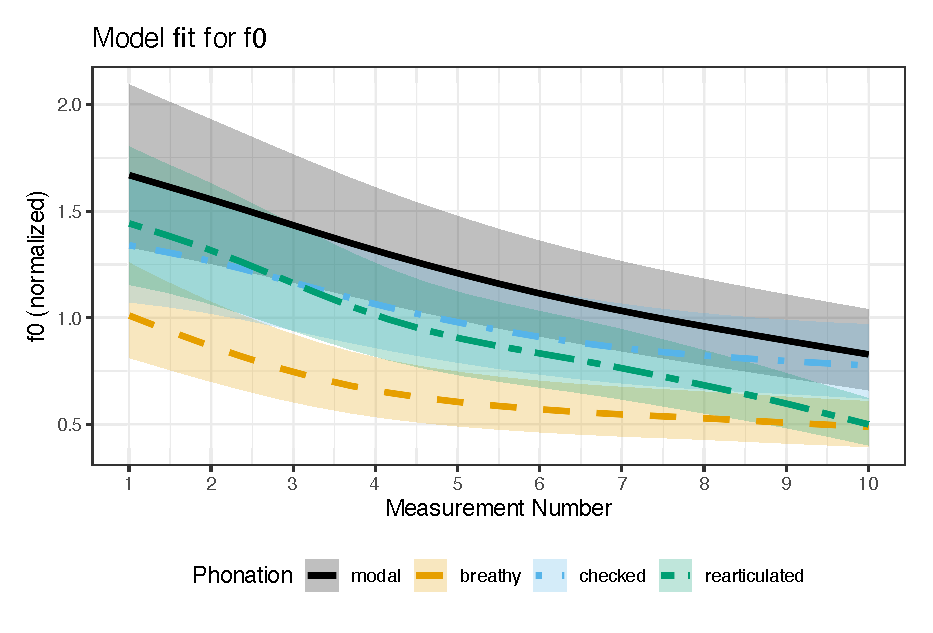
\includegraphics[width = 0.8\linewidth]{images/LCH_GAMMs/f0_model_fit.eps}
  \end{figure}
\end{frame}

\begin{frame}{Difference plots for \textit{f}0}
  \begin{figure}
    \centering
    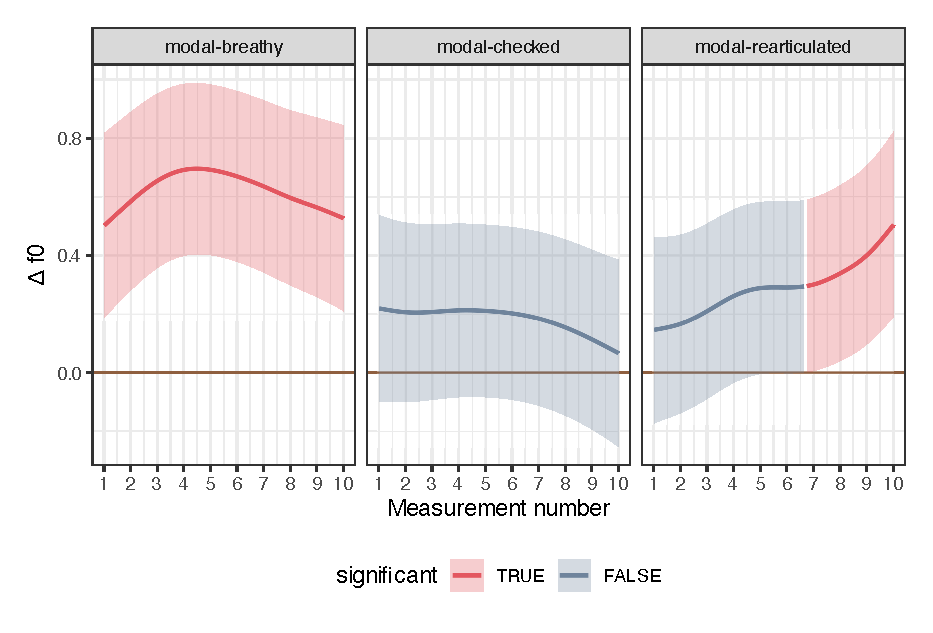
\includegraphics[width = 0.8\linewidth]{images/LCH_GAMMs/f0_model_diff.eps}
  \end{figure}
\end{frame}

\begin{frame}{Model fit for HNR}
  \begin{figure}
    \centering
    \includegraphics[width = 0.8\linewidth]{images/LCH_GAMMs/hnr15_model_fit.eps}
  \end{figure}
\end{frame}

\begin{frame}{Difference plots for HNR}
  \begin{figure}
    \centering
    \includegraphics[width = 0.8\linewidth]{images/LCH_GAMMs/hnr15_model_diff.eps}
  \end{figure}
\end{frame}

\begin{frame}{Model fit for SoE}
  \begin{figure}
    \centering
    \includegraphics[width = 0.8\linewidth]{images/LCH_GAMMs/soe_model_fit.eps}
  \end{figure}
\end{frame}

\begin{frame}{Difference plots for SoE}
  \begin{figure}
    \centering
    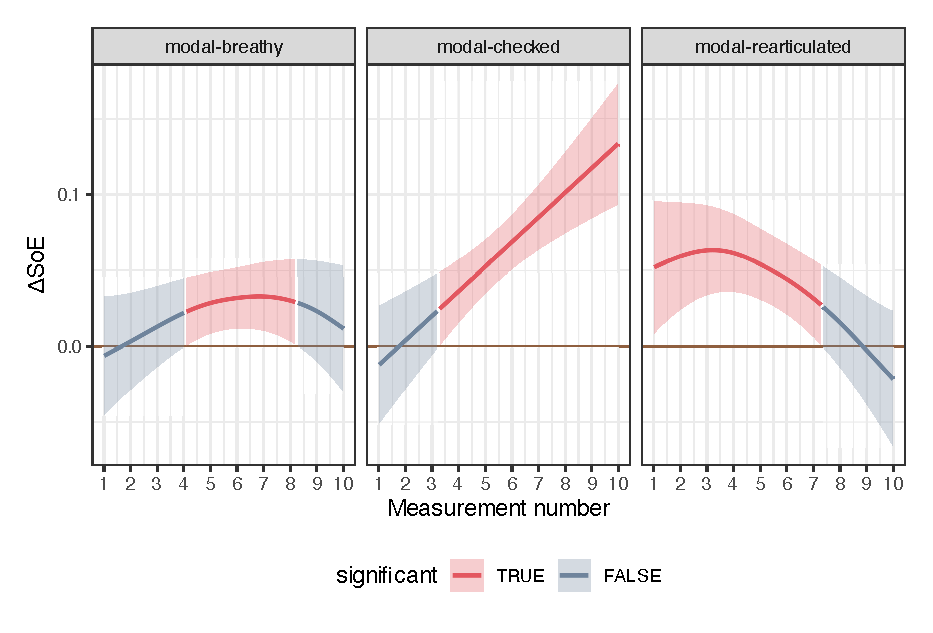
\includegraphics[width = 0.8\linewidth]{images/LCH_GAMMs/soe_model_diff.eps}
  \end{figure}
\end{frame}

\begin{frame}{Summary of Laryngeal Complexity}
  \begin{itemize}
    \item SLZ shows phasing.
    \begin{itemize}
      \item Breathy shows postvocalic phasing.
      \item Checked shows postvocalic phasing.
      \item Rearticulated shows prevocalic phasing.
      \item No evidence for interrupted phasing. 
    \end{itemize}
    \item Implicational hierarchy of laryngeal complexity holds.
    \item Laryngealization is weakly articulated in SLZ.
  \end{itemize}
\end{frame}

%-----------------------------------------------------------
\section{Summary and conclusions}
%-----------------------------------------------------------
\begin{frame}{Summary of Research Questions}
\begin{block}{Research Questions:}
    \begin{itemize}
      \item How is phonation's acoustic space structured in a single language?
      \item Which measures are important for capturing phonation contrasts?
      \item How do these measures help explain SLZ's laryngeal complexity?
    \end{itemize}
  \end{block}
\end{frame} 

\begin{frame}{Summary of Answers}
  \begin{block}{Answers to Research Questions:}
    \begin{itemize}
      \item The acoustic space is three-dimensional and correlated with glottal-airflow (D1/D3) and nonmodal-to-modal (D2) continua.
      \item Only a handful of measures are needed for capturing contrasts.
      \item SLZ's laryngeal complexity is weakly articulated and shows phasing. 
    \end{itemize} 
  \end{block}
\end{frame}

\begin{frame}{Implications and big picture}
  \begin{itemize}
    \item Showcases \posscitet{keatingCrosslanguageAcousticSpace2023} methodology for narrowing down which acoustic measures to use.
    \item Analysis is congruent with \posscitet{keatingCrosslanguageAcousticSpace2023} findings.
    \item SLZ's phonation is consistent with \posscitet{silvermanLaryngealComplexityOtomanguean1997} claims about laryngeal complexity.
    \item Shows that HNR and SoE are useful measures for quantifying laryngeal complexity.
  \end{itemize}
\end{frame}

\begin{frame}{Next steps}  
  % The following outlook is optional.
  \begin{itemize}
    \item What are the perceptual cues that SLZ speakers use to distinguish phonation types?
    \item How do the dimensions of the acoustic space relate to phonological features?
    \item Do we actually observe interrupted phasing in other Zapotec languages?
    \item How do we analyze laryngeal complexity's phasing patterns in the phonology?
  \end{itemize}
\end{frame}

\begin{frame}
  \frametitle{\textit{Duxhklhenhu' lhe'} (Thank you all!)}
  \begin{figure}
    \centering
    \includegraphics[width = \linewidth]{images/SantiagoLaxopa.jpeg}
  %   \label{fig:fieldwork}
  \end{figure}
\end{frame}

%-----------------------------------------------------------
\section*{Acknowledgements}
%-----------------------------------------------------------

\begin{frame}
  \frametitle{Acknowledgements}
  \begin{itemize}
    \item Thank you to Maestra Fe Silva-Robles for introducing me and teaching me about \textit{Dille'xhunh}
    \item Thank you to the other speakers of \textit{Dille'xhunh} for sharing their time and language expertise. 
    \item Thank you to Grant McGuire, Jaye Padgett, Marc Garellek, Ryan Bennett, Jack Duff, Maya Wax Cavallaro, and many others for their help and discussions during all stages of this project. 
  \end{itemize}
\end{frame}

\begin{frame}
  \frametitle{Acknowledgements}
  This work is supported by funding from: 
  \begin{itemize}
    \item The National Science Foundation under Grant No. 2019804
    \item The Humanities Institute at UC Santa Cruz 
    \item The Jacobs Research Funds
  \end{itemize}

\end{frame}


\appendix
%-----------------------------------------------------------
\section<presentation>*{\appendixname}
%-----------------------------------------------------------
%-----------------------------------------------------------
\section{References}
%-----------------------------------------------------------
\begin{frame}[t,allowframebreaks]
  \frametitle{References}
    \printbibliography
\end{frame}

%-----------------------------------------------------------
\section{Acoustic Measures from MDS}
%-----------------------------------------------------------
\begin{frame}[t,allowframebreaks]{Correlations of Acoustic Measures to Dimensions}
  \small
  \begin{longtable}{lrrrr}
    \lsptoprule
    \textbf{Acoustic Measure} & \textbf{NMDS1} & \textbf{NMDS2} & \textbf{NMDS3} & \textbf{NMDS4} \\
    \midrule
    H1*$-$H2* & -0.221 & -0.339 & 0.031 & 0.314 \\
    H2*$-$H4 & -0.437 & 0.239 & \textbf{-0.689} & \textbf{-0.364} \\
    H1*$-$A1* & \textbf{-0.828} & 0.048 & \textbf{-0.459} & 0.044 \\
    H1*$-$A2* & \textbf{-0.855} & -0.067 & -0.343 & 0.114 \\
    H1*$-$A3* & \textbf{-0.809} & -0.218 & -0.297 & 0.126 \\
    H4*$-$H2k* & -0.452 & -0.598 & 0.294 & \textbf{0.366} \\
    H2k*$-$H5k* & 0.152 & 0.023 & 0.101 & 0.057 \\
    residual H1* & -0.290 & -0.443 & \textbf{-0.722} & 0.084 \\
    H2* & -0.157 & -0.555 & \textbf{-0.679} & 0.114 \\
    H4* & 0.295 & \textbf{-0.778} & 0.078 & \textbf{0.479} \\
    A1* & 0.756 & -0.549 & 0.092 & 0.124 \\
    A2* & \textbf{0.779} & -0.476 & -0.103 & 0.086 \\
    A3* & 0.735 & -0.416 & -0.211 & 0.093 \\
    \lspbottomrule
  \end{longtable}

  \begin{longtable}{lrrrr}
    \lsptoprule
    \textbf{Acoustic Measure} & \textbf{NMDS1} & \textbf{NMDS2} & \textbf{NMDS3} & \textbf{NMDS4} \\
    \midrule
    CPP & -0.590 & -0.606 & 0.209 & -0.179 \\
    HNR < 500 Hz & -0.513 & \textbf{-0.792} & 0.152 & -0.202 \\
    HNR < 1500 Hz & -0.275 & \textbf{-0.799} & 0.323 & -0.290 \\
    HNR < 2500 Hz & -0.327 & -0.714 & 0.391 & -0.348 \\
    HNR < 3500 Hz & -0.446 & -0.644 & 0.393 & -0.356 \\
    Strength of Excitation & -0.013 & -0.741 & -0.238 & 0.145 \\
    SHR & 0.144 & -0.176 & 0.122 & \textbf{-0.597} \\
    Energy & -0.080 & \textbf{-0.793} & -0.015 & 0.341 \\
    Duration & -0.622 & 0.539 & 0.257 & 0.030 \\
    \lspbottomrule
  \end{longtable}
\end{frame}

%-----------------------------------------------------------
\section{Acoustic Measures from Random Forest}
%-----------------------------------------------------------


\begin{frame}{Duration}
  \begin{figure}
    \centering
    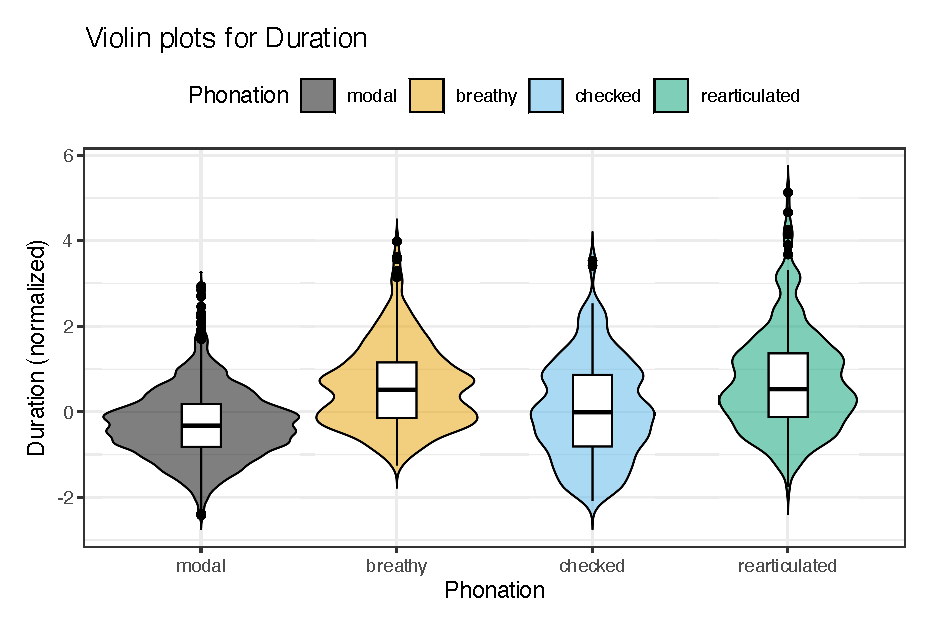
\includegraphics[width = 0.8\linewidth]{images/duration_plot.eps}
  \end{figure}
\end{frame}

\begin{frame}{A1*}
  \begin{figure}
    \centering
    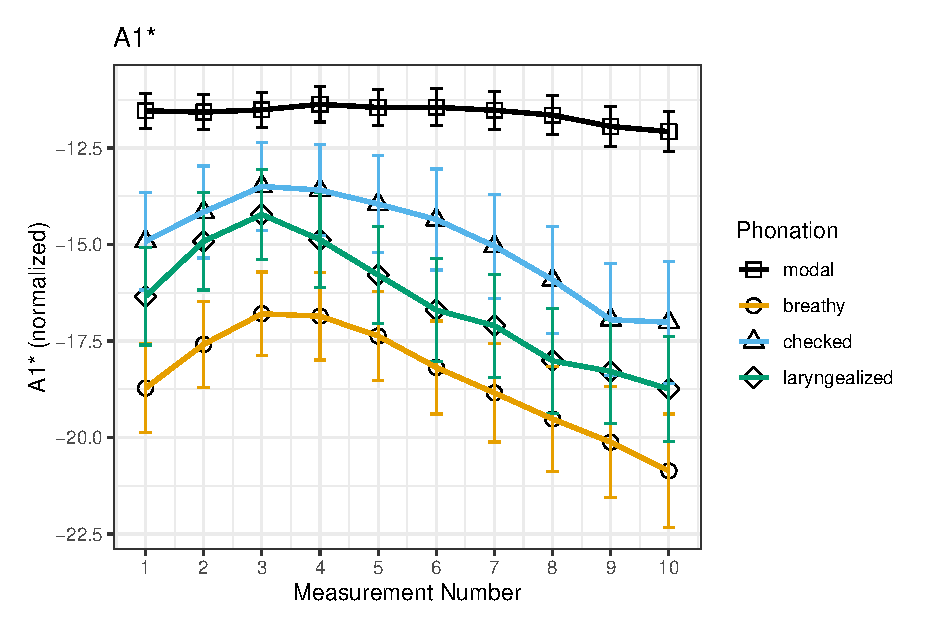
\includegraphics[width = 0.8\linewidth]{images/slz_a1c.eps}
  \end{figure}
\end{frame}

\begin{frame}{H1*$-$A1*}
  \begin{figure}
    \centering
    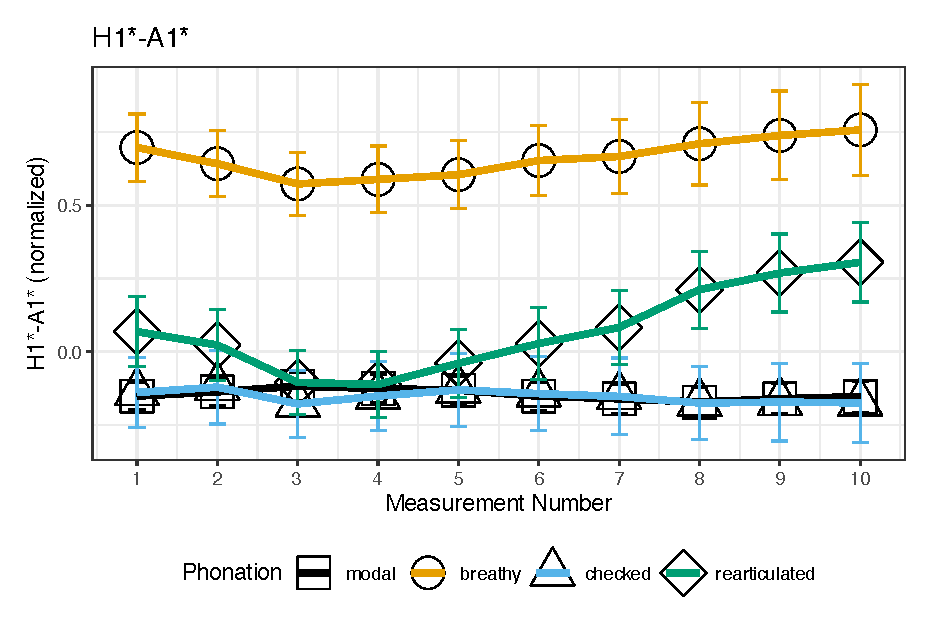
\includegraphics[width = 0.8\linewidth]{images/h1a1_line.eps}
  \end{figure}
\end{frame}

\begin{frame}{Residual H1*}
  \begin{figure}
    \centering
    \includegraphics[width = 0.8\linewidth]{images/slz_residual_h1c.eps}
  \end{figure}
\end{frame}

\begin{frame}{HNR < 1500 Hz}
  \begin{figure}
    \centering
    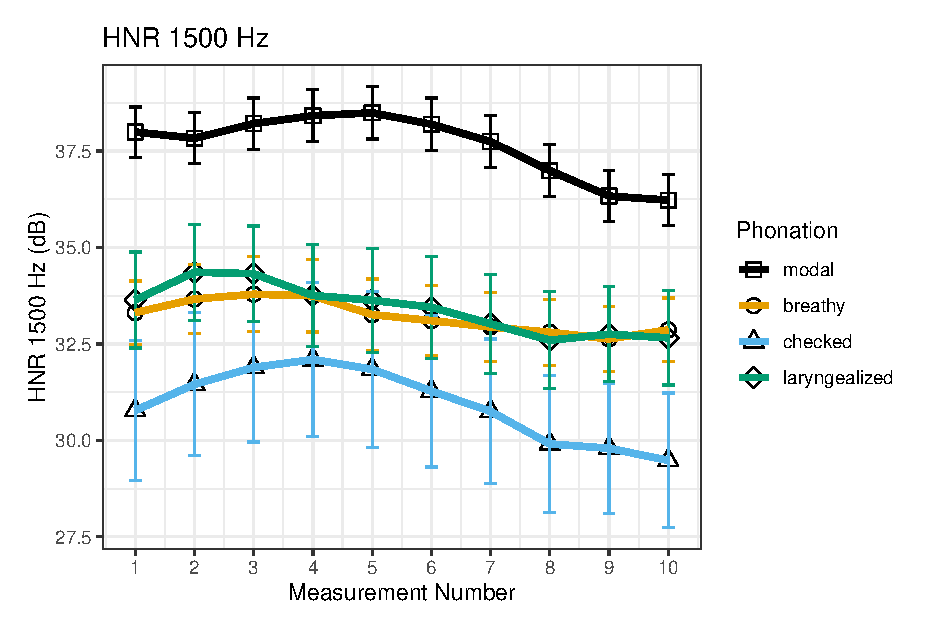
\includegraphics[width = 0.8\linewidth]{images/slz_hnr15.eps}
  \end{figure}
\end{frame}

\begin{frame}{Strength of Excitation (SoE)}
  \begin{figure}
    \centering
    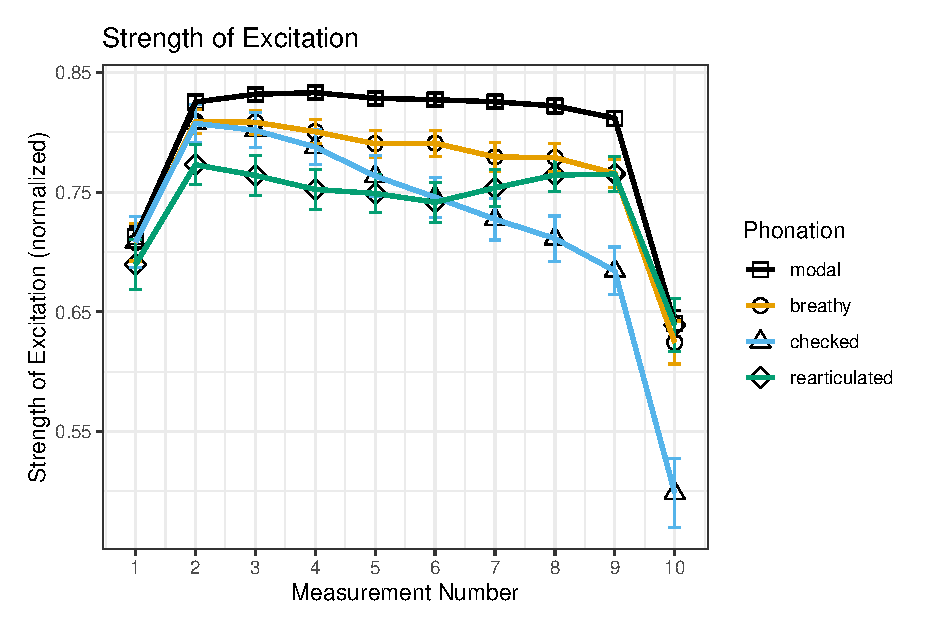
\includegraphics[width = 0.8\linewidth]{images/slz_soe.eps}
  \end{figure}
\end{frame}

\end{document}